\chapter{Theory}


\section{Machine Learning}

Due to the advancement in the field of Artificial Intelligence (AI), the ability to tackle entire problems of machine intelligence. Nowadays, Machine Learning (ML) is becoming a hot topic due to the direct training of machines with less interaction with a human. The scenario of manually feeding the machine is changing in the modern era, it will learn automatically. The methods of learning can be roughly categorized into two main groups - supervised learning and unsupervised learning. Nowdays we know of other methods like reinforcement learning, semi-supervised learning, and many hybrid approaches.

\subsection{Supervised Learning}
When the data takes the form of input variables and target values for the output, supervised learning is used. The mapping function from the input to the output is learned by the algorithm. It's a costly method for problems where data is limited since large-scale labeled data samples are available. 
 \begin{itemize}[]
 	\item Classification\\
 	One of a known number of categories is represented by the output variable. For instance, "dog" or "cat," "positive" or "negative."
 	\item Regression\\
 	The value of the output variable is continuous or actual. For instance, "geographical location," "price,"
 \end{itemize}

\subsection{Unsupervised Learning}
podporne vektory, k means, dbscan

\section{Neural Networks}
An artificial intelligence technique called a neural network trains computers to process information in a manner similar to that of the human brain. It uses connected nodes or neurons arranged in a layered pattern to mimic the organization of the human brain. Computers can utilize this adaptive approach to learn from their errors and keep getting better. As a result, artificial neural networks make an effort to more accurately answer challenging problems, such as document summarization and face recognition.


Neurons are small, basic building components of neural networks. Each neuron takes inputs which it processes and outputs it as an input for next neuron. Neurons in the input layer, as well as in the output layer are defined. The neuron connections carry weights. The higher the weight, the bigger impact to the other neuron that is connected. A neuron normally takes the mean value of the connected neurons based on the connection weights. All neurons have transfer function, that determines whether or not to accept the triggered inputs from the connected neurons. The neuron decides, sets its value, and triggers the next neurons with that value.
The value that the transfer function typically returns is a mix of the neuron's triggered value and current value. The majority of the work is done by the hidden neurons. However, as we are only concerned with the input and output neurons and are unaware of what occurs in the neurons between them, we refer to them as hidden neurons. That being said, most neural networks are multilayered, which means there are also hidden layers of neurons besides the input and output neurons.

\begin{figure}[htp]
	\centering
	\begin{tikzpicture}[
		>=Stealth,
		input/.style={},
		weights/.style={},
		neuron/.style={
			circle,
			draw,
			thick,
			minimum size=1cm,
			fill=white
		},
		function/.style={
			rectangle,
			draw,
			thick,
			minimum size=1cm
		}
		]
		
		% Inputs
		\node[input] (Input-1) at (0,-1) {$x_1$};
		\node[input] (Input-2) at (0,-2) {$x_2$};
		\node[input] (Input-n) at (0,-3) {$x_n$};
		\node at (0,-2.4) {$\vdots$};
		
		% Weights
		\node[weights] (Weights-1) at (2,-1) {$w_1$};
		\node[weights] (Weights-2) at (2,-2) {$w_2$};
		\node[weights] (Weights-n) at (2,-3) {$w_n$};
		
		% Arrows for weights
		\draw[->, thick] (Input-1) -- (Weights-1);
		\draw[->, thick] (Input-2) -- (Weights-2);
		\draw[->, thick] (Input-n) -- (Weights-n);
		
		% Summation circle
		\node[neuron] (Sum) at (4, -2.5) {$\sum$};
		
		% Bias
		\node[input] (Bias) at (4,-4) {$b$};
		
		% Activation function
		\node[function] (Activation) at (6, -2.5) {$f$};
		
		% Output
		\node[input] (Output) at (8, -2.5) {$\hat{y}$};
		
		% Arrows from weights and bias to sum
		\foreach \i in {1,2,n} {
			\draw[->, thick] (Weights-\i.east) -- (Sum.west);
		}
		\draw[->, thick] (Bias) -- (Sum);
		
		% Arrow from sum to activation function
		\draw[->, thick] (Sum) -- (Activation);
		
		% Arrow from activation function to output
		\draw[->, thick] (Activation) -- (Output);
		
	\end{tikzpicture}
	
	\caption{Schematic representation of a neuron with inputs, weights, a bias, an activation function, and an output.}
	\label{fig:neuron}
\end{figure}



\begin{figure}[htp]
	\centering
	\begin{tikzpicture}[
		plain/.style={
			draw=none,
			fill=none,
		},
		dot/.style={draw,shape=circle,minimum size=3pt,inner sep=0,fill=black
		},
		net/.style={
			matrix of nodes,
			nodes={
				draw,
				circle,
				inner sep=8.5pt
			},
			nodes in empty cells,
			column sep=0.6cm,
			row sep=-11pt
		},
		>=latex
		]
		\matrix[net] (mat)
		{
			|[plain]| \parbox{1cm}{\centering Input\\layer} 
			& |[plain]| \parbox{1cm}{\centering Hidden\\layer} 
			& |[plain]| \parbox{1cm}{\centering Output\\layer} \\
			& |[plain]|                 \\
			|[plain]| &            & |[plain]|    \\
			& |[plain]|  &              \\
			|[plain]| & |[dot]|                   \\
			& |[plain]|  & |[dot]|      \\
			|[plain]| & |[dot]|    & |[plain]|    \\
			|[dot]|   & |[plain]|  & |[dot]|      \\
			|[dot]|   & |[dot]|    & |[plain]|    \\
			|[dot]|   & |[plain]|  &              \\
			|[plain]| &            & |[plain]|    \\
			& |[plain]|                 \\
		};
		\foreach \ai/\mi in {2/I1,4/I2,6/I3,12/In}
		\draw[<-] (mat-\ai-1) -- node[above] {\mi} +(-1cm,0);
		\foreach \ai in {2,4,6,12}
		{\foreach \aii/\mii in {3/H1,11/Hm}
			\draw[->] (mat-\ai-1) -- (mat-\aii-2) node[yshift=0.6cm] {\mii};
		}
		\foreach \ai in {3,11}
		{  \draw[->] (mat-\ai-2) -- (mat-4-3);
			\draw[->] (mat-4-3) -- node[above] {O1} +(1cm,0);}
		\foreach \ai in {3,11}
		{  \draw[->] (mat-\ai-2) -- (mat-10-3);
			\draw[->] (mat-10-3) -- node[above] {Op} +(1cm,0);}
	\end{tikzpicture}
	
	\caption{Structure of neural network}
	\label{neural_n_example}
\end{figure}
 
 
 
\subsection*{Activation Functions}
A weighted sum of signals received from the neurons on the preceding layer is fed into neuron's activation function. After that, the activation function's output is passed onto next layer of the network.
These are main types of activation function used: threshold, sigmoid, rectifier, hyperbolic tangent, softmax


\subsubsection*{Threshold Function}
The output signal computed by threshold functions varies based on whether the input is above or below a predefined threshold. 

The formal definition of a deep learning threshold function in mathematics is as follows:

\begin{equation}
f(x) =
\begin{cases}
	0 & \text{if } x < 0,\\
	1 & \text{if } x \geq 0
\end{cases}
\end{equation}



\begin{figure}[htp]
	\centering
\begin{tikzpicture}
	% Axes
	\draw[-stealth] (-pi,0) -- (pi,0) node[right]{$x$};
	\draw[-stealth] (0,0) -- (0,2) node[above]{$y$};
	% Plot
	\draw[thick, blue] (-pi,0) -- (0,0) -- (0,1) -- (pi,1);
	% Numbers
	\node[below] at (0,0) {$0$}; % x=0
	\node[left] at (0,1) {1}; % y=1
\end{tikzpicture}
\end{figure}


The threshold function is sometimes referred to as a unit step function, as the image above illustrates. In computer programming, threshold functions are comparable to boolean variables. Their calculated value is either 0 (which is equal to False) or 1 (which is comparable to True).


\subsubsection*{Sigmoid Function}
The data science community is familiar with the sigmoid function from its application in logistic regression. It tells us the probability of whether a 

Any value can be entered into the sigmoid function, but it will always return a value between 0 and 1.

The sigmoid function has the following mathematical definition:

\begin{equation}
	\sigma(z) = \frac{1} {1 + e^{-z}}
\end{equation}

For evaluating a single metric (feature) the sigmoid function has threshold value of 0.5 for binary decisions. 

\begin{figure}[htp]
	\centering
\begin{tikzpicture}
	\begin{axis}[
		axis lines=middle,
		xmax=10,
		xmin=-10,
		ymin=-0.05,
		ymax=1.05,
		xlabel={$x$},
		ylabel={$y$}
		]
		\addplot [domain=-9.5:9.5, samples=100,
		thick, blue] {1/(1+exp(-x)};
	\end{axis}
\end{tikzpicture}
\label{sigmoid function}
\caption{sigmoid}
\end{figure}

The smoothness of the sigmoid function's curve gives it an advantage over the threshold function. This implies that derivatives can be computed at any point on the curve.


\subsubsection*{Rectifier  Function}
Unlike the sigmoid function from, the rectifier function does not have the same smoothness property. It is still  highly used in the deep learning community.

The definition of the rectifier function outputs 0 if the input value is less than 0. The function outputs the input if it isn't. It helps to maintain mathematical stability and keep learned values from being stuck around 0 or jumping into infinity.



\begin{equation}
	Relu(x) = max(0, x)
\end{equation}
\begin{figure}[htp]
	\centering
\begin{tikzpicture}
	\begin{axis}[
		axis lines=middle,
		xmax=6,
		xmin=-6,
		ymin=-0.05,
		ymax=5.05,
		xlabel={$x$},
		ylabel={$y$}]
		\addplot [domain=-5.5:5.5, samples=100, thick, blue] {max(0, x)};
	\end{axis}
\end{tikzpicture}
\end{figure}


Rectified Linear Unit activation functions, or ReLUs for short, are a common term for rectifier functions. 


\subsubsection*{Hyperbolic Tangent Function
}
The activation function  based on a trigonometric identity is the hyperbolic tangent function. Below is its mathematical definition:

\begin{equation}
	\varphi(x) = \tanh(x) = \frac{\sinh(x)}{\cosh(x)} = \frac{e^x - e^{-x}}{e^x + e^{-x}}
\end{equation}
\begin{figure}[htp]
	\centering
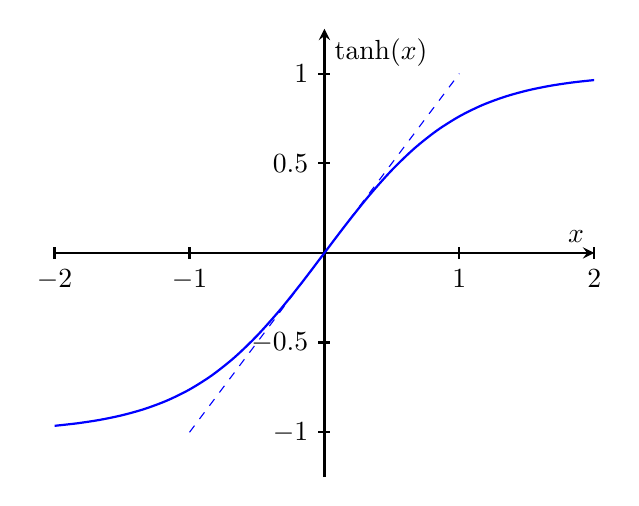
\begin{tikzpicture}
	\begin{axis}[
		xlabel = $x$,
		ylabel = $\tanh(x)$,
		ymin = -1.25,ymax = 1.25,
		domain = -2:2,
		smooth,thick,
		axis lines = center,
		every tick/.style = {thick}]
		
		\addplot[color=blue]{tanh(x)};
		\addplot[color=blue,dashed,domain=-1:1,thin]{x};
		
	\end{axis}
\end{tikzpicture}
\end{figure}


The hyperbolic tangent function resembles the sigmoid function, but all of its output values are shifted down.


\subsubsection*{SoftMax Function
}
An activation function called Softmax is used to convert numbers or logits (outputs of neural network) into probabilities. A vector  containing the probabilities of every possible result is the result of a Softmax. The vector's  probabilities add up to one for every possible outcome or class.

\begin{equation}
	\sigma(z_i) = \frac{e^{z_{i}}}{\sum_{j=1}^K e^{z_{j}}} \ \ \ for\ i=1,2,\dots,K
\end{equation}

\begin{figure}[htp]
	\centering
	\begin{tikzpicture}[
		box/.style={
			draw, 
			thick, 
			rectangle, 
			minimum height=1cm, 
			minimum width=1.2cm, % Reduced width of boxes
			text width=1.2cm,      % Reduced text width inside boxes
			align=center,
			scale=0.8,           % Scale down everything inside the boxes
		},
		node distance=0.5cm,     % Reduced distance between nodes
		scale=1.2,               % Scale the entire tikzpicture
		every node/.style={transform shape} % This ensures that the scaling affects all nodes
		]
		
		% Define nodes
		\node[box] (image) {image of a bird};
		\node[box, right=of image] (layers) {layers of NN};
		\node[box, right=of layers, text width=1.5cm] (logits) {2.5\\1.3\\0.2\\4.6};
		\node[box, right=of logits] (softmax) {softmax function};
		\node[box, right=of softmax, text width=1.5cm] (probabilities) {0.75\\0.19\\0.02\\0.04};
		\node[box, right=of probabilities, text width=1.5cm] (classes) {Bird\\Mouse\\Cat\\Worm};
		
		% Connect nodes
		\draw[-stealth] (image) -- (layers);
		\draw[-stealth] (layers) -- (logits);
		\draw[-stealth] (logits) -- (softmax);
		\draw[-stealth] (softmax) -- (probabilities);
		\draw[-stealth] (probabilities) -- (classes);
		
		% Add titles above boxes
		\node[above=1mm of logits] {Logits};
		\node[above=1mm of probabilities] {Probabilities};
		\node[above=1mm of classes] {Classes};
		
	\end{tikzpicture}
	\caption{A diagram of the NN softmax classification process.}
\end{figure}

\subsection{Feedforward Neural Network}
Weights are assigned after an input layer has been identified. Larger weights contribute more significantly to the output than smaller ones, helping to determine the relative importance of each variable. After that, each input is multiplied by its corresponding weight before being added together. The output is then determined by passing it through an activation function. The node "fires," or activates, when its output surpasses a predetermined threshold, forwarding data to the network's subsequent layer. As a result, one node's output ends up becoming the next node's input. This neural network is classified as a feedforward network because of the way that data is passed from one layer to the next.


\subsection{Training A Neural Network}
The weights of the connections between the nodes are randomly chosen, and neural networks then use a technique known as backpropagation to learn new, improved connection weights based on the inputs and outputs that are predetermined. Neural networks can therefore learn.
The random connection weights are used after the inputs and outputs are selected. Next, the output is computed and evaluated relative to the expected outputs. The difference is referred to as a network error.  The error should be to be minimal. Backpropagation is used for that purpose.  The connected neurons receive a message about their error from the output neurons, and the connection weight between them is modified. The weights are computed using a learning rate, errors, neuron inputs, and the previous weight.\\
%Backpropagation
\subsubsection*{Cost functions}

 As we train the model, we’ll want to evaluate its accuracy using a cost (or loss) function. Loss function tells us about how good our algorithm models our dataset.The loss error is calculated for each training sample, while the loss function represents the whole set of $m$ samples. The cost function represents the average loss error for each sample. It is a function that assesses how well a machine learning model performs with a given set of data. The error between expected and predicted values is quantified by the Cost Function and shown as a single real number. Cost functions can be formed in a variety of ways, depending on the nature of the problem. For a model using a formula 
 \begin{equation*}
 	\hat{y} = wx
 \end{equation*}, where $\hat{y}$ is predicted value, $x$ a vector of data used for prediction and training and $w$ the weight.
 
  
 The commonly used loss function is the mean squared error (MSE).  In the equation below,

$i$ represents the index of the sample,
$\hat{y}$ is the predicted outcome,
$y$ is the actual value, and
$m$ is the number of samples.

\begin{equation}
 MSE = \frac{1}{2m} \sum_{i=1}^{m} (\hat{y}^{(i)} - y^{(i)})^2
\end{equation}


Crossentropy function
Other names for cross-entropy loss include logistic loss, log loss, and logarithmic loss. Every predicted class probability is compared to the actual class probability, and a loss function is used to penalize the probability according to its deviation from the actual expected value. Because the penalty is logarithmic, large differences near to 1 will result in a large score, and small differences approaching 0 will result in a small score. Cross-entropy loss in a perfect model is 0.
What is meant by cross-entropy is 
\begin{equation}
		-\sum_{c=1}^My_{o,c}\log(p_{o,c})
\end{equation}
where $M$ is number of classes, $y$ is the binary indicator if class of label $c$ is the correct classification for observation $o$ and $p$ is the predicted probability.

When dealing with labels that are one-hot encoded, such as in the case of the 3-class classification problem, where the values are [1,0,0], [0,1,0], and [0,0,1], categorical cross-entropy is employed.
Labels in sparse categorical cross-entropy are encoded with integers, such as [1], [2], and [3] for a 3-class problem.


There are many other types of cost functions used in ML, e.g. Root Mean Square error (RMSE), Binary Cross Entropy Loss Function,  Categorical cross-entropy, Hinge Loss, Kullback-Liebler Divergence LOSS (KL-Divergence), Huber Loss. Choosing a cost function will be influenced by the type of problem, the output activation function and network architecture.


When talking about regulation of neural networks we can mention techniques like dropout or early stopping.

Dropout is a regularization strategy for neural networks that, with a given probability p, drops a unit (along with connections) during training.
The goal is to stop co-adaptation, which occurs when a neural network becomes overly dependent on a single connection and may be an indication of overfitting. It makes intuitive sense to think of dropout as the formation of an implicit neural network ensemble.

\def\layersep{2}
\def\nodesep{1.5}
\begin{figure}[htp]
	\centering
	\begin{tikzpicture}[
		node/.style={circle, draw, thick},
		scale=0.8, % Adjust the scaling factor as needed
		transform shape,
		every node/.style={scale=0.8} % Adjust the node text scaling factor as needed
		]
	
	\foreach \y in {1,...,5}{
		\node[node] (i\y) at (0,\nodesep*\y) {};
		\node[node, right=\layersep of i\y] (h1\y) {};
		\node[node, right=\layersep of h1\y] (h2\y) {};
	}
	
	\node[node, right=\layersep of h22] (o1) {};
	\node[node, right=\layersep of h24] (o2) {};
	
	\foreach \source in {1,...,5}
	\foreach \dest in {1,...,5}{
		\path[-stealth, thick] (i\source) edge (h1\dest);
		\path[-stealth, thick] (h1\source) edge (h2\dest);
	}
	\foreach \source in {1,...,5}
	\foreach \dest in {1,2}
	\draw[-stealth, thick] (h2\source) -- (o\dest);
	
	\draw[-stealth, thick] (7.5,3*\nodesep) -- node[above,font=\Large] {dropout} (9.5, 3*\nodesep);
	
	% Boundary
	
	\foreach \y in {1,...,5}
	\node[node, right=15em of h2\y] (di\y) {};
	
	\node[red,font=\huge] at (di1) {$\times$};
	\node[red,font=\huge] at (di3) {$\times$};
	
	\foreach \y in {1,...,5}
	\node[node, right=\layersep of di\y] (dh1\y) {};
	
	\node[red,font=\huge] at (dh11) {$\times$};
	\node[red,font=\huge] at (dh13) {$\times$};
	\node[red,font=\huge] at (dh14) {$\times$};
	
	\foreach \y in {1,...,5}
	\node[node, right=\layersep of dh1\y] (dh2\y) {};
	
	\node[red,font=\huge] at (dh22) {$\times$};
	\node[red,font=\huge] at (dh24) {$\times$};
	
	\node[node, right=\layersep of dh22] (do1) {};
	\node[node, right=\layersep of dh24] (do2) {};
	
	\foreach \source in {2,4,5}
	\foreach \dest in {2,5}
	\draw[-stealth, thick] (di\source) -- (dh1\dest);
	
	\foreach \source in {2,5}
	\foreach \dest in {1,3,5}
	\draw[-stealth, thick] (dh1\source) -- (dh2\dest);
	
	\foreach \source in {1,3,5}
	\foreach \dest in {1,2}
	\draw[-stealth, thick] (dh2\source) -- (do\dest);
	
\end{tikzpicture}
\end{figure}

An intuitive technique for training just enough, is early stopping. It prevents the model from learning on 'noised' dataset. When training, after every epoch, the model is evaluated using a validation dataset. The training process is terminated if the model's performance on the validaion dataset begins to drop (for example, if loss starts to rise or accuracy starts to fall).



\subsection*{Hyperparameters of Neural Networks}
\begin{itemize}
	\item Learning Rate is a crucial parameter that controls to which extend the model needs to be modified. It is determines the step size at each training iteration. It is usually a value between 0 and 1. We can determine the direction of a loss function's optimum by computing the loss function's gradient. The step size that  in that direction is determined by the learning rate parameter.
	\item Batch size tells us how much data is changed during 1 cycle (one epoch) of training. Larger batch sizes could lead to faster training, but with a trade off for lower accuracy or overfitting. The best size will depend on a number of variables, such as the size of the training dataset, the complexity of the model, and the available computational resources.
	\item Epochs define the number times that the learning algorithm will work through the entire training dataset. Every sample in the training dataset has had a chance to update the internal model parameters after one epoch. One or more batches make up an epoch.
\end{itemize}



\subsection*{Optimalizators of Neural Networks}
\begin{itemize}
	\item Gradient Descent
	\item Stochastic Gradient Descent
	\item Adam
\end{itemize}


%for a neural network 
%how, training, gradient zostup, chybova funkcia, hyperparameter
%types - feed forward, recurrent, lstm, kohonens self organizing maps
%aktivacne funkcie - skryte/vstupne/vystupne; krokova, linearna, sigmoid, tanh, relu, leaky relu, softmax, ,Dropout, hyperparameter?, rychlost ucenia - learning rate, epochs, batch size, optimalizators - fradient descent, stochastic gd, adam, EarlyStopping, sparse categorical crossentropy',
%our opencv library



\section{Techniques used in Computer Vision }

In Computer Vision (CV), ML plays an important role in extracting important information from images. CV successfully contributes to various domains, surveillance system, optical character recognition, robotics, suspect detection, and many more.  The direction of CV research is going towards healthcare domain, medical imaging (MI) is the emerging technology, play a vital role to improve image quality and recognized critical features of binary medical image, covert original image into grayscale and set the threshold for segmentation.
Within computer vision, three key tasks stand out: segmentation, detection, and classification. 
\subsection*{Image Classifiaction}
	It's a known fact that the image we see as a whole is made up of hundreds to thousands of tiny pixels. Before computer vision can determine and label the image as a whole, it needs to analyze the individual components of the image. That is why image classification techniques analyze a given image in the form of pixels and accomplish this by treating the picture as an array of matrices, the size of which is determined by the image resolution. The pixels of the digital image are taken and grouped into what we know as “classes.” From this point on, the procedure will vary depending on the algorithm. To guarantee that it is not left entirely on the final classifier, the selected algorithm will convert the image into a series of key attributes. These characteristics aid the classifier in identifying the subject matter and class to which the image belongs. 
	We can say that the image classification pipeline looks like this:
	image pre-processing -> feature extraction -> object classification
	
	
	Based on the nature of the problem, there are different types of image classification methodologies. They are binary, multiclass, multilabel, and hierarchical.
	
	Binary classification divides unknown data points into two groups using an either-or logic for labeling images. Binary classification is used to handle many different yes/no problems, such as analyzing product quality to determine whether a product has faults, and many more tasks requiring judgment calls.
	
	As the name implies, multiclass divides objects into three or more classes, whereas binary classification divides objects into two classes. It's highly helpful in a variety of fields, including medical diagnostics (disease categorization), NLP (sentiment analysis in situations involving several emotions), etc.
	 
	The multilabel method permits an object to be allocated to more than one label, in contrast to multiclass classification, which assigns an image to a single class. For instance, you could have to categorize multiple colors in an image. Taking a picture of a  salad, a picture of one will feature red, orange, yellow, purple, and other colors. Consequently, several colors will be used as labels on a single image.
	
	The process of classifying classes into a hierarchical structure based on their similarities is known as hierarchical classification. A lower-level class is more definite and detailed, while a higher-level class represents larger categories. If we're classifying a dog, our first model would recognize dog vs other animal. If a dog is correctly predicted, another model will be used to classify the breed of the dog into border collie, golden retriever, poodle. All features of higher-class attributes will be hierarchically contained in the latter ones. Hierarchy allows for effective information transfer between related classes as well as a flexible and interpretable framework for organizing and representing complex visual concepts.
	

Image Classification correlates one class from the training data with a whole image or video frame regardless of the amount of information present. It involves assigning labels, is suitable when fine-grained information is not necessary. During the model training stage, publically accessible datasets are frequently employed to enable correct data labeling.
\subsection*{Object Detection}
	The classification is advanced in object detection. It not only classifies many objects in an image, but also provides annotations for the bounding boxes that correspond to each entity's position. The CV model's extra benefits enable its implementation in a number of practical contexts as these models are only a small portion of detecting, labeling, and annotating objects in images or videos. Faster R-CNN, YOLO (You Only Look Once), and SSD (Single Shot MultiBox Detector) are a few popular object detection algorithms. These algorithms are tailored to specific application requirements and differ in terms of speed, accuracy, and trade-offs.  An example of an object detection model is a model for human detection. Model would return a bounding box around each person with a label
	
	\begin{figure}[ht]
		\centering
		\begin{minipage}{0.4\textwidth}
			\centering
			\includegraphics[width=0.7\linewidth]{images/cat_class.jpg}
				\caption*{Cat}
			\label{fig:justcat}
		\end{minipage}% <-- Add this percentage sign here
		\begin{minipage}{0.48\textwidth}
			\centering
			\includegraphics[width=0.7\linewidth]{images/catanddog_detect.jpg}
				\caption*{Cat, Dog}
			\label{fig:catanddog}
		\end{minipage}
		\caption{Comparison of classification (left) with output: 'Cat' and object detection (right) with output: 'Cat, Dog' and their localization with bounding boxes }
		\label{fig:both_figures_class_detect} % This label can now be used to reference both images together
	\end{figure}
	
	

	\subsection*{Image Segmantation}

	Since they both serve the same purpose, object detection and image segmentation are comparable. Both techniques identify items in pictures and provide coordinates for locating objects. However, segmentation algorithms produce accurate masks that cover objects at the pixel level, as opposed to creating whole boxes around them.
	
	Annotations for image segmentation include the exact pixel locations of any instances that are present in the image. Image segmentation is better suitable for practical uses because of its accurate results. However, compared to object detection, picture segmentation models are computationally expensive due to algorithm complexity.
	The example use is in applying  visual effects like background blurring and makup effects to the image. The functionality identifies specific textures, colors and segments object features within image data. It is also widely used ub medical imaging, self-driving cars or satelite imaging. 
	
In the figure figxx a U-Net, an architecture introduced by Olaf Ronneberger, Philipp Fischer and Thomas Brox in 2015 is used. It's a convolutional neural network that was specifically designed to be used in Biomedical Imaging. A pretrained model MobileNetV2 is used as a lightweight, efficient feature extractor for the input image. It would analyze the photo of the dog and create a set of feature maps highlighting important visual attributes like edges, textures, and shapes relevant for the segmentation task. Then, with the feature maps provided by MobileNetV2, U-Net would take on the task of image segmentation. Its architecture, designed to work with fewer data points and to be precise in delineating object boundaries, would use the feature maps to generate a predicted mask. It would attempt to closely replicate the true mask by classifying each pixel as belonging to the dog or the background. A Pix2Pix model is then used to generate a segmented image that tries to match the true mask, learning the mapping from the input image to the segmentation mask during training.
	
	For this task it is also possible to use interactive segmantation, which devides image into two regions: selected object and everything else.It receives a location in an image, calculates the object's boundaries at that location , and returns image data that defines the object's area. 



\begin{figure}[ht]
	\centering
	\begin{minipage}{0.3\textwidth}
		\centering
		\includegraphics[width=0.9\linewidth]{images/pose_landmarks_index.png}
	%	\caption{Landmarks for pose estimation model by MediaPipe}
		\label{fig:pose_landmarks}
	\end{minipage}% <-- Add this percentage sign here
	\begin{minipage}{0.48\textwidth}
		\centering
		\includegraphics[width=\linewidth]{images/dog.png}
	%	\caption{U-Net segmentation on an image from Oxford-IIIT Pet Dataset (Parkhi et al, 2012).}
		\label{fig:dog}
	\end{minipage}
	\caption{Landmarks for pose estimation model by MediaPipe and U-Net segmentation on an image from Oxford-IIIT Pet Dataset (Parkhi et al, 2012).}
	\label{fig:both_figures} % This label can now be used to reference both images together
\end{figure}



%types of models
%neural networksas

%use and so on, how works
%rgb gbr conversion

%\section{Types of classifiers and models for Computer Vision}
%An algorithm, or the set of rules that robots employ to classify data, is called a classifier. %However, the final result of the classifier's machine learning is a classification model. The %data is first classified by the model, which was trained using the classifier. 


\section{Mediapipe}
MediaPipe is a framework used to create machine learning pipelines for time-series data like video and audio. Google initially developed it to process real-time video and audio analysis on YouTube. In 2019, the public release allowed researchers and developers to incorporate MediaPipe into their projects. Unlike other machine learning frameworks that require high computing power, MediaPipe can run efficiently on devices with low power, such as Android and IoT devices. It consists of the MediaPipe framework and MediaPipe solutions. The MediaPipe framework is developed using C++, Java, and Objective C programming. MediaPipe solutions include 16 pre-trained TensorFlow and TensorFlow Lite models built on top of the MediaPipe framework for specific use cases. 


\subsection*{MediaPipe Hands}
The problem of detecting hands is somewhat intricat. The model must be able to recognize hands and it must function across a wide range of hand sizes with a big scale span so it must be robust. It is rather difficult to identify hands based just on their visual traits since hands lack the high contrast patterns.% found on faces, such as those surrounding the lips and eyes.


MediaPipe Hands is a solution that tracks hands in real-time. MediaPipe Hands utilizes a combination of object detection, classification and regression to recognize and track hands within a given image or video frame. The pipeline consists of two models: palm detector and a hand landmark model.


The palm detector is a single-shot detector model  that uses a orientated hand bounding box to locate palms on a whole input image. This is done before landmark detection because it is easier to estimate bounding boxes of rigid objects like palms than detecting hands with articulated fingers. It ignores many aspect ratios and so the bounding boxes are only squared. The model uses both classification (hands, no hands), and object detection (predicting a bounding box around the detected hand). 


The Hand Landmark Model runs subsequently with the palm detection model and uses regression to precisely localize 21 3D coordinates within the hand region. Each landmark has a specific location on the hand that can vary within the pixel grid of an image. To capture the exact position, continuous values are used, allowing the model to indicate precisely where each landmark is located on the hand in terms of its x and y (and possibly z) coordinates within the image. As the hands move and rotate freely, leading to a wide range of possible positions and orientations for each landmark,  Continuous outputs enable the model to track these changes smoothly and accurately across frames in real-time.
The model is resilient to self-occlusions and partially visible hands, and it learns a consistent internal hand posture representation. The results form the model contain 21 hand landmarks consisting of x, y, and z, a hand flag that indicates the likelihood that a hand is present in the input image and a binary system of handedness, e.g. left or right hand. 
The coordinates x and y for each landmark are normalize to [0, 1] by image width and height. See more in Data Normalization.

The model was trained both on real-world and synthetic datasets, noting that the wrist point being learned only from synthetic images. More than 30,000 manually annotated real-world images were used and the model is very robust, allowing it to detect and map hand landmark points accurately, even on partially visible hands in most cases. In 
\ref{fig:landmark_both_hands} my hands are not facing upfront but the model still finds all the landmarks for both hands. If tracking 2 hands, it also shows which one is left or right with different colors.

For encountering a tracking failure, There was also another model output created for tracking failures. It generates the likelihood that the given crop actually contains a hand that is reasonably aligned. The detector is triggered to reset tracking if the score falls below a predetermined threshold. 

\begin{figure}
	\centering
	\includegraphics[width = 0.5\textwidth]{images/landmarks_both_hands.png}
	\caption{Hand landmarks model output}
	\label{fig:landmark_both_hands}
\end{figure}

\subsubsection*{Data Normalization}
The MediaPipe hand landmarks model provides coordinates for hand landmark points based on the position of pixels containing those points in an image. As a result, the coordinates of two images of the same hand sign with different placements in the frame can have significantly different distances between them. This makes it more challenging to train the model.

To solve this problem, the wrist's landmark point has been considered with coordinates [0,0], and the coordinates of all other landmark points were adjusted accordingly.
First, the coordinates' values of the wrist's landmark point are subtracted from all coordinates' values. 

Then, the coordinates were normalized to be between 0 and 1 by dividing them by the largest absolute value of the difference. Finally, the normalized coordinates were collected in the landmarks list. The coordinate normalization procedure is shown in Fig \ref{fig:normalization}.


\begin{figure}
	\centering
	\includegraphics[width = 0.85\textwidth]{images/normalise.pdf}
	\caption{Process of normalization of landmark coordinates}
	\label{fig:normalization}
\end{figure}

\subsection*{MediaPipe Face}
With support for multiple faces and six landmarks (left eye, right eye, nose tip, mouth, left eye tragion, and right eye tragion), MediaPipe Face Detection  a quick solution for face detection. BlazeFace, a compact and efficient face detector designed for mobile GPU inference, serves as its foundation. Because of its real-time performance, the detector can be used with any live viewfinder experience that needs a precise facial region of interest as an input for other task-specific models, like face region segmentation, facial feature or expression classification, and 3D facial keypoint estimation (like MediaPipe Face Mesh). BlazeFace leverages an enhanced tie resolution technique as an alternative to a GPU-friendly anchor mechanism adapted from Single Shot MultiBox Detector (SSD), and a lightweight feature extraction network that is similar to but different from MobileNetV1/V2. 


\begin{figure}[ht]
	\centering
	\begin{minipage}{0.5\textwidth}
		\centering
		\includegraphics[width=0.5\textwidth]{images/face_detection_good.png}
		%   \caption{Landmarks for pose estimation model by MediaPipe}
	\end{minipage}% <-- This percentage sign denotes the end of a minipage
	\begin{minipage}{0.5\textwidth}
		\centering
		\includegraphics[width=0.5\textwidth]{images/face_detection.png}
		%   \caption{U-Net segmentation on an image from Oxford-IIIT Pet Dataset (Parkhi et al, 2012).}
	\end{minipage}
	\caption{Outputs of face detection model with different lightings}
	\label{fig:face_detections} % This label can now be used to reference both images together
\end{figure}



The Hand 
company, availability, types of models, what they offer, devices options, what we use

%\subsection{Input Image Processing}
%color, background, extracting landmarks for mediapipe model no. 2, with vs without Mediapipe






\section{Gesture Recognition}

The process of recognizing hand gestures as input, mapping them to a representation, and converting them into a purposeful command for devices is known as gesture recognition. The goal is to identify and process explicit hand gestures for output. 
Dynamic gestures refer to a sequence of poses that change over time, while static gestures remain constant. Static hand gestures can be classified based on their temporal relationship and recognized by analyzing features such as spatial position, orientation, contour, and texture. We will focus on recognizing static gestures using a vision-based method.

%tu nejake obrazky na classification

\section{Drone Control}



